\documentclass{article}
\usepackage[utf8]{inputenc}
\usepackage{graphicx}
\title{Ein dynamischer Access-Point-Ansatz für Smart-Home-Anwendungen}

\author{Michael Jathe}
\date{März 2021}

\begin{document}

\maketitle

\section{Einleitung}

\subsection{Motivation}

Der Smart Home Sektor befindet sich seit Jahren in
einem stetigen Wachstum. Die Zahl der Hersteller von
Smart Home Produkten nimmt zu und die Automatisierung
und Überwachung breitet sich auf alle Bereiche
im Haus aus.\\

Wichtige Aspekte des Smart Homes sind die Kommunikation
zwischen den Sensoren/Aktoren, die Anbindung an das
Internet und die Steuerung per Smartphone.\\

Viele Hersteller haben ihr eigenes System
entwickelt. Für die Anbindung der Sensoren und Aktoren
wird ein eigener Access Point benötigt. Der Datenaustausch
findet über Funk, WLAN oder Ethernet und ein Herstellereigenes
Protokoll statt. Für die Internetanbindung wird
meist eine eigene Cloudlösung angeboten oder der Access
Point wird über Portfreigaben von Außen erreichbar gemacht,
was ein erhebliches Sicherheitsrisiko mit sich bringt. Ein
Vorteil dieser Systeme ist die einfache und kostengünstige
Nachrüstung.\\

Da sich die Hersteller nicht auf einen gemeinsamen Standard
geeinigt haben, sind die Systeme von verschiedenen
Herstellern meist nicht miteinander kompatibel. Daher müssen
sich die Nutzer entweder auf das Produktangebot eines Herstellers
beschränken oder für jeden weiteren Hersteller einen
zusätzlichen Access Point installieren. Zudem wird für jedes System
eine eigene App zur Nutzerinteraktion benötigt.\\

Ziel dieser Arbeit ist es, einen Ansatz für dynamische Access Points zu entwickeln. Alle Knoten im Netzwerk sollen zur Laufzeit die Funktion des Access Points übernehmen können. Als Anwendugnsbeispiel soll ein System zur Pflanzen- und Raumluftüberwachung dienen. 
\subsection{Anforderungen}
\begin{itemize}
    \item Das System muss ohne dedizierten Acces Point auskommen.
    \item Jeder Knoten muss auch als Access Point/Broker fungieren können.
    \item Bei Ausfall des Access Points/Brokers wird muss das System selbständig einen neuen Broker bestimmen.
    \item Bei Ausfall des Brokers darf kein Datenverlust entstehen.
    \item Der Broker muss die gesammelten Sensordaten in einen Cloudspeicher übertragen
    \item Die Daten müssen über eine Weboberfläche oder App abrufbar sein.

\end{itemize}
\subsection{Konzept}
Es soll ein System entwickelt werden, in dem jeder Knoten, das heißt Sensor, Aktor oder Bedienelement, auch die Funktion des Access Point übernehmen kann. Für die Kommunikation wird MQTT(Message Queuing Telemetry Transport) eingesetzt. MQTT ist ein offenes Netzwerkprotokoll für Machine-to-Machine-Kommunikation (M2M), das die Übertragung von Telemetriedaten in Form von Nachrichten zwischen Geräten ermöglicht.
MQTT beruht auf dem Client-Server-Modell. Der Server, auch Broker genannt, stellt den Clients Kanäle zur Kommunikation zur Verfügung. Die Clients können diese Kanäle anlegen, auf Ihnen Nachrichten veröffentlichen und sie abonnieren, um Nachrichten von anderen Clients zu empfangen. 
\\

Bei der Konfiguration des ersten Knoten/Clients wird dieser als Broker festgelegt. Alle weiteren Clients melden sich bei dem Broker an. Der Broker legt eine Tabelle mit allen Clients und deren IP-Adressen an. Sobald sich ein neuer Client anmeldet, wird die aktualisierte IP-Tabelle an alle Clients gesendet. Das geschieht über einen MQTT-Kanal dem alle Clients folgen.

\begin{figure}[h]
    \centering
    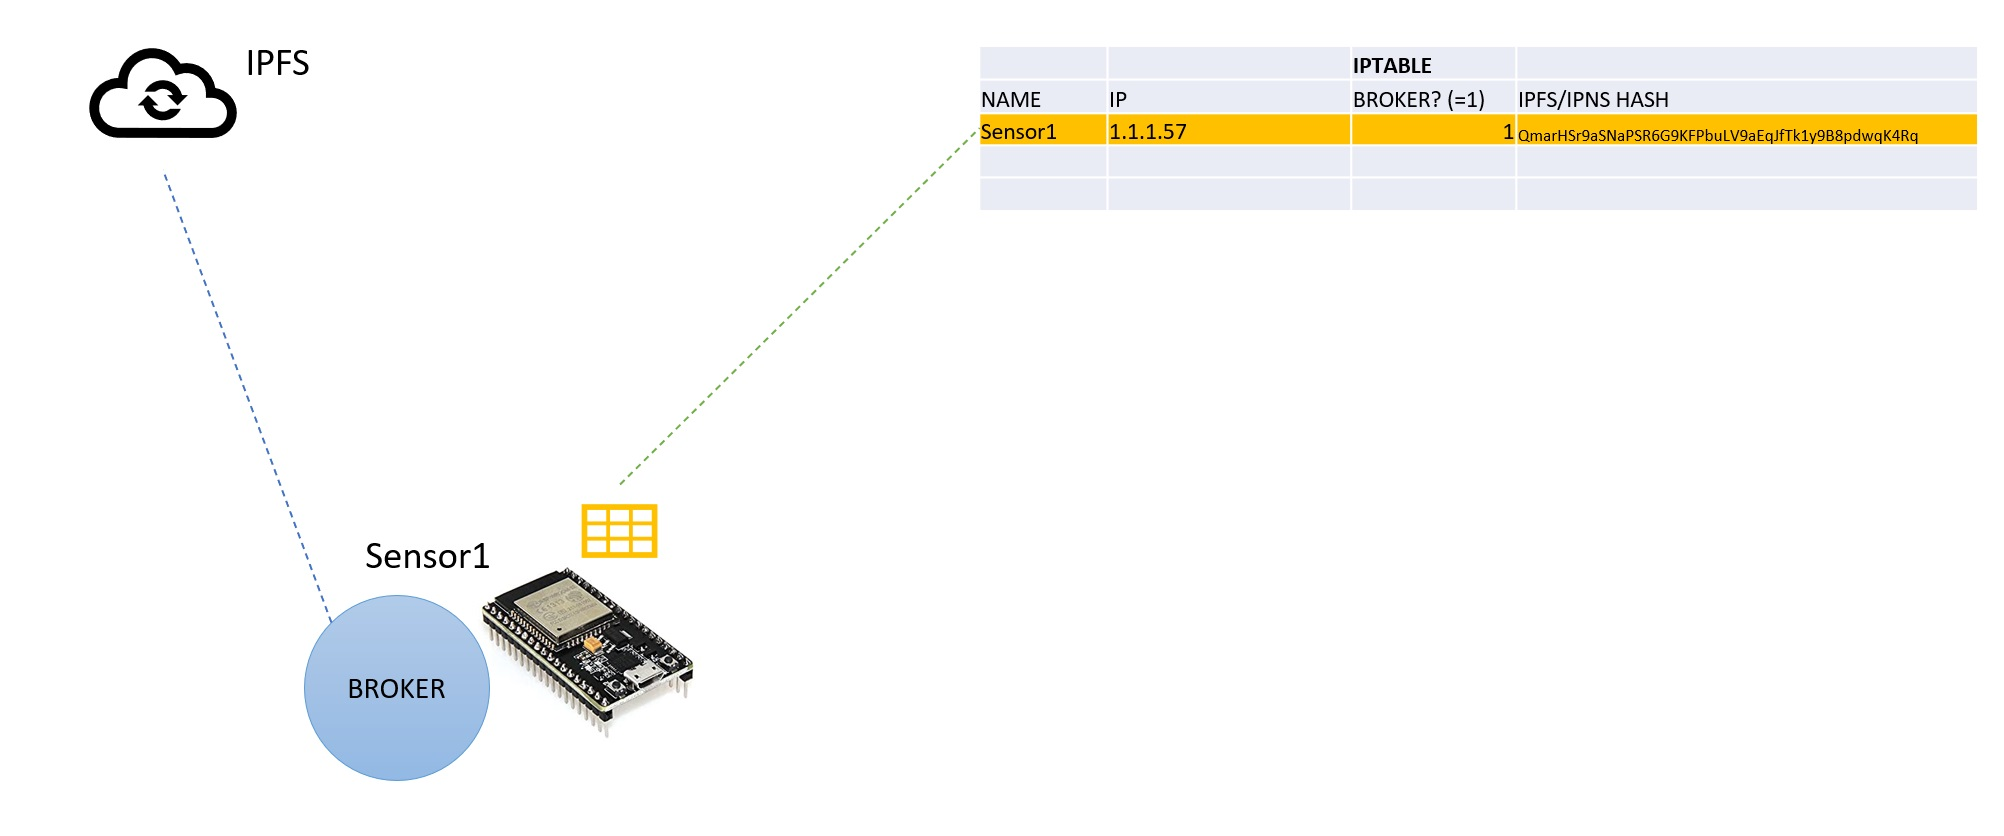
\includegraphics[width=1\linewidth]{Porposal/Bilder/bild1.jpg}
    \caption{Der erste Client wird Broker und erstellt die IP-Tabelle}
    \label{fig:statemachine}
\end{figure}

Der zweite und alle weiteren Clients melden sich beim Broker an und bekommen die aktualisierte IP-Tabelle gesendet. Sollte der Broker die Verbindung verlieren, übernimmt der Client mit der niedrigsten IP-Adresse die Rolle des Brokers. Da alle Clients immer die aktuelle IP-Tabelle haben, weiß jeder Client unter welcher IP der neue Broker erreicht werden kann. Zusätzlich wird die IP-Tabelle noch auf dem Cloudspeicher abgelegt, damit sich der alte Broker mit dem neuen verbinden kann. Sollte durch den Absturz die IP-Tabelle verloren gegangen sein, muss das Gerät neu konfiguriert werden.

\begin{figure}[h]
    \centering
    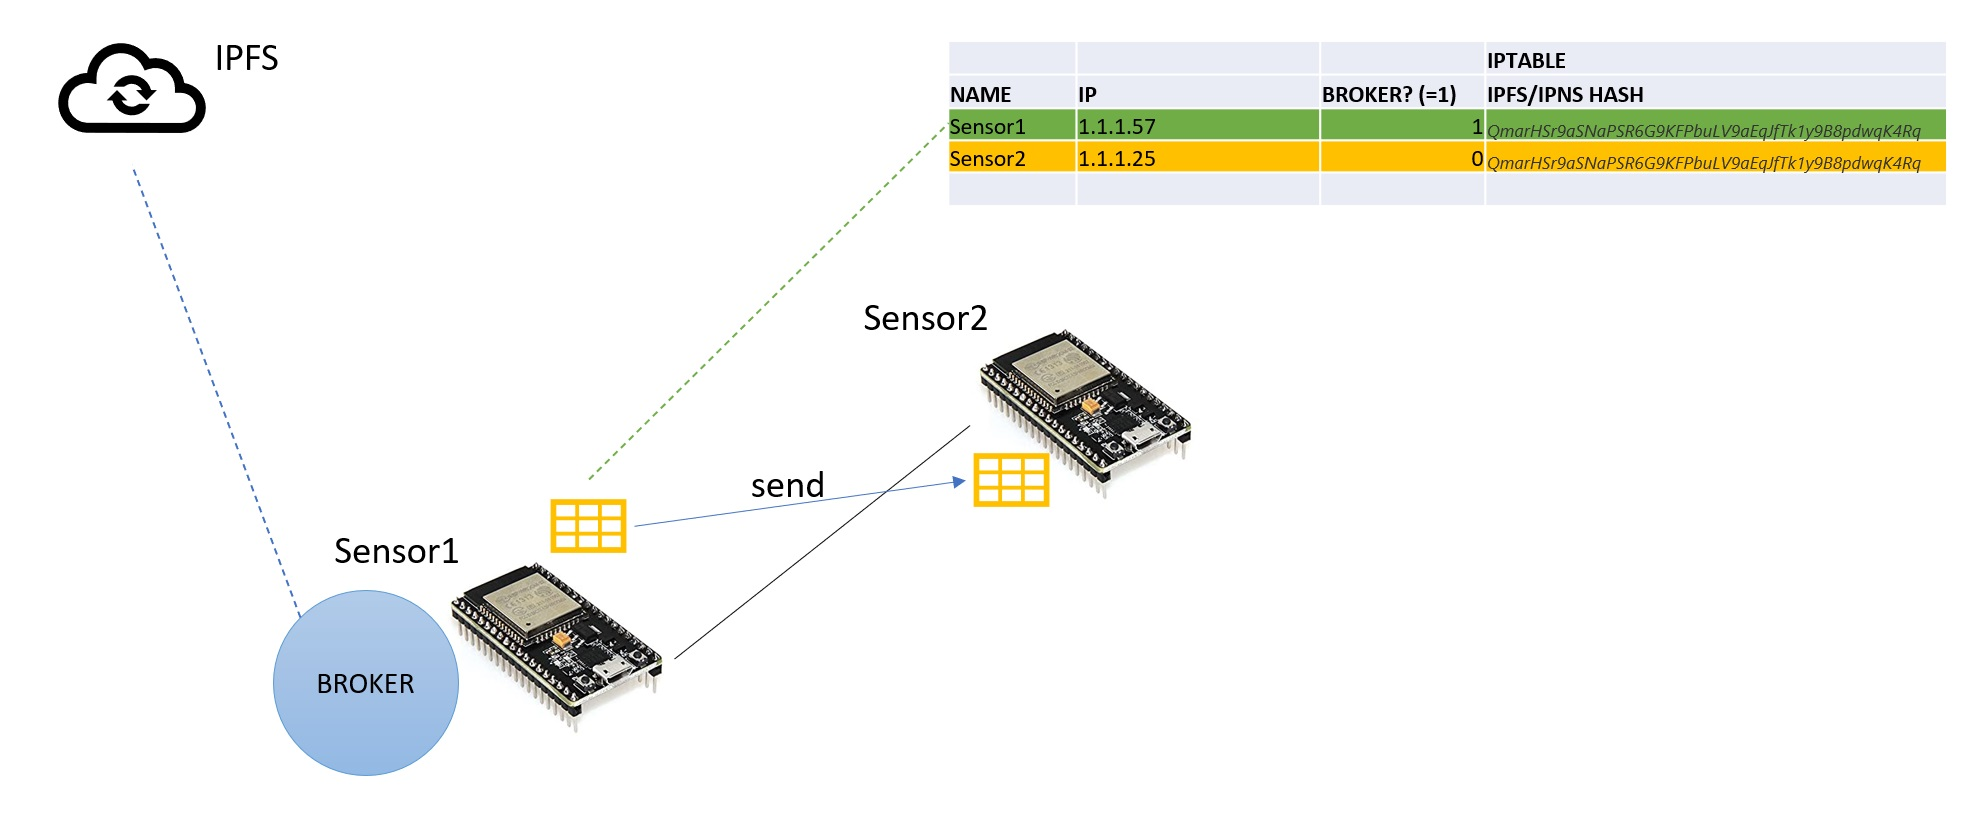
\includegraphics[width=1\linewidth]{Porposal/Bilder/bild2.jpg}
    \caption{Der zweite Client meldet sich beim Broker an und bekommt die aktuelle IP-Tabelle.}
    \label{fig:statemachine}
\end{figure}

Der Broker hat außerdem die Aufgabe, alle Daten der Clients zu sammeln und diese kurzen Abständen in einem Cloudspeicher zu hinterlegen. 
\begin{figure}[h]
    \centering
    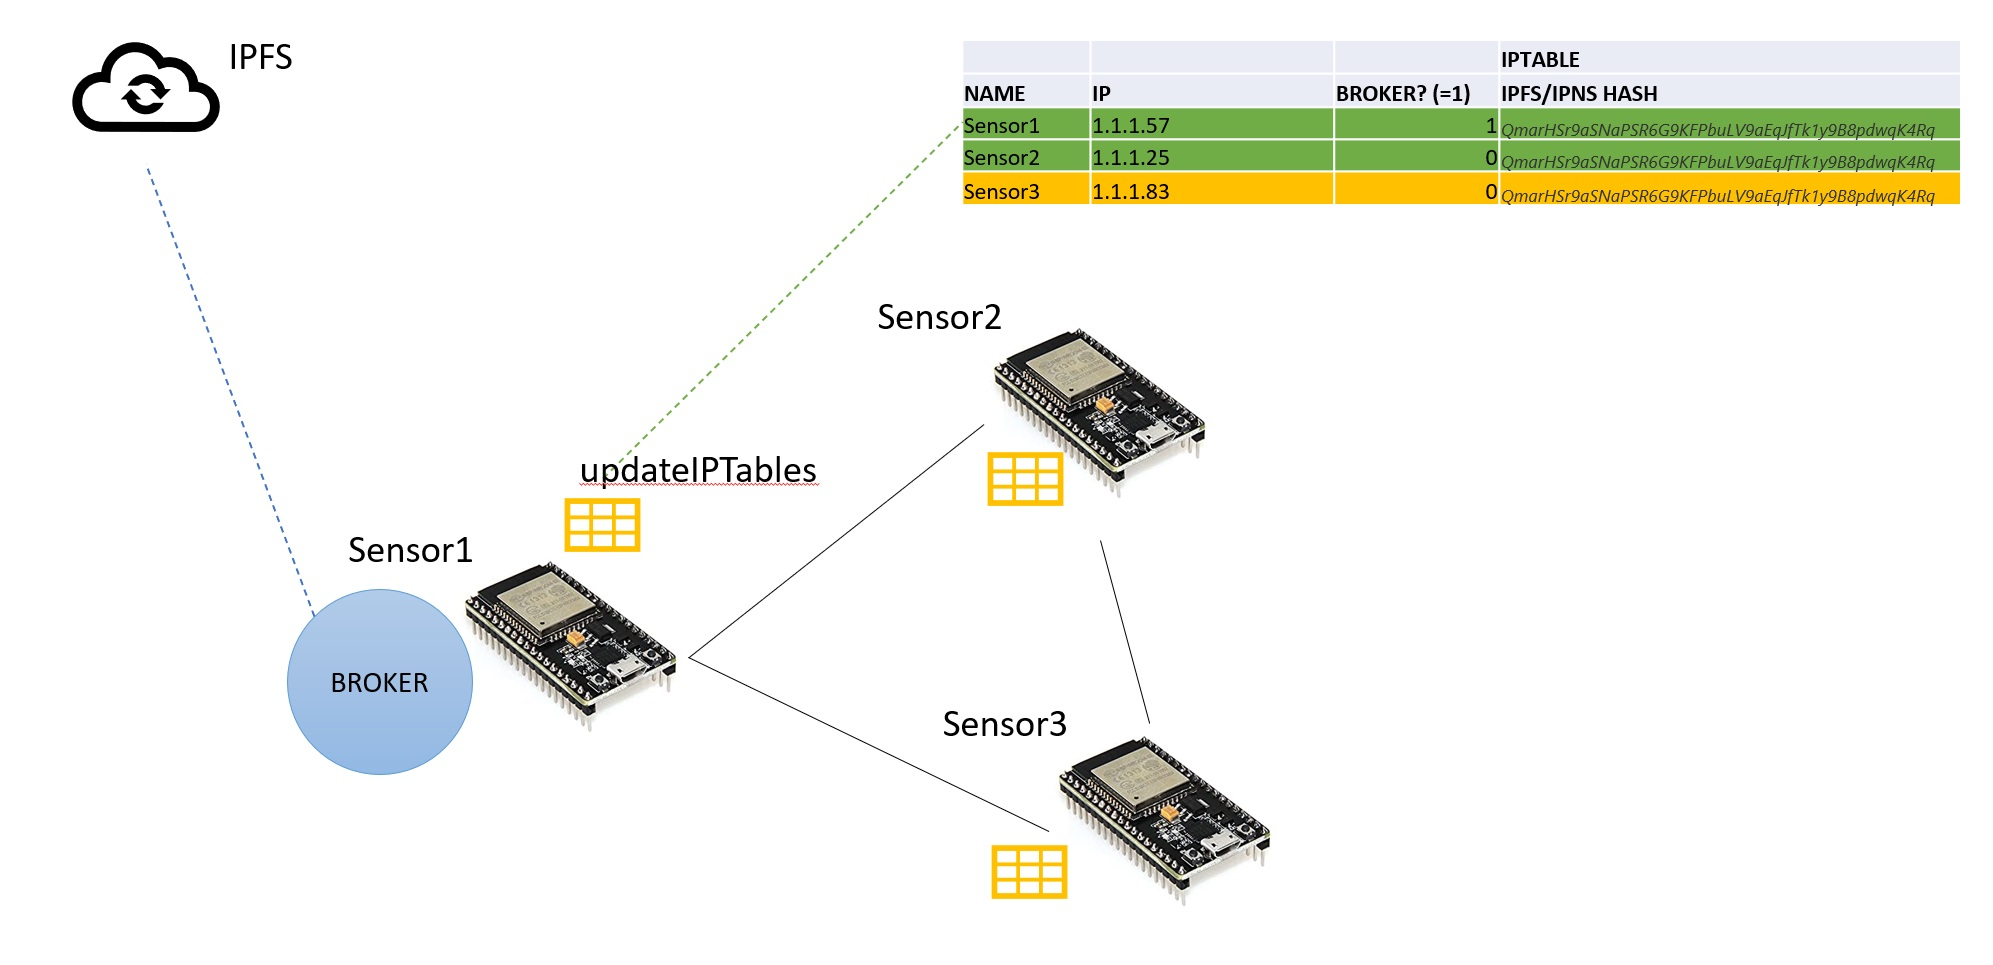
\includegraphics[width=1\linewidth]{Porposal/Bilder/Bild3.jpg}
    \caption{Der dritte Client meldet sich beim Broker an und bekommt die aktuelle IP-Tabelle.}
    \label{fig:statemachine}
\end{figure}
\begin{figure}[h]
    \centering
    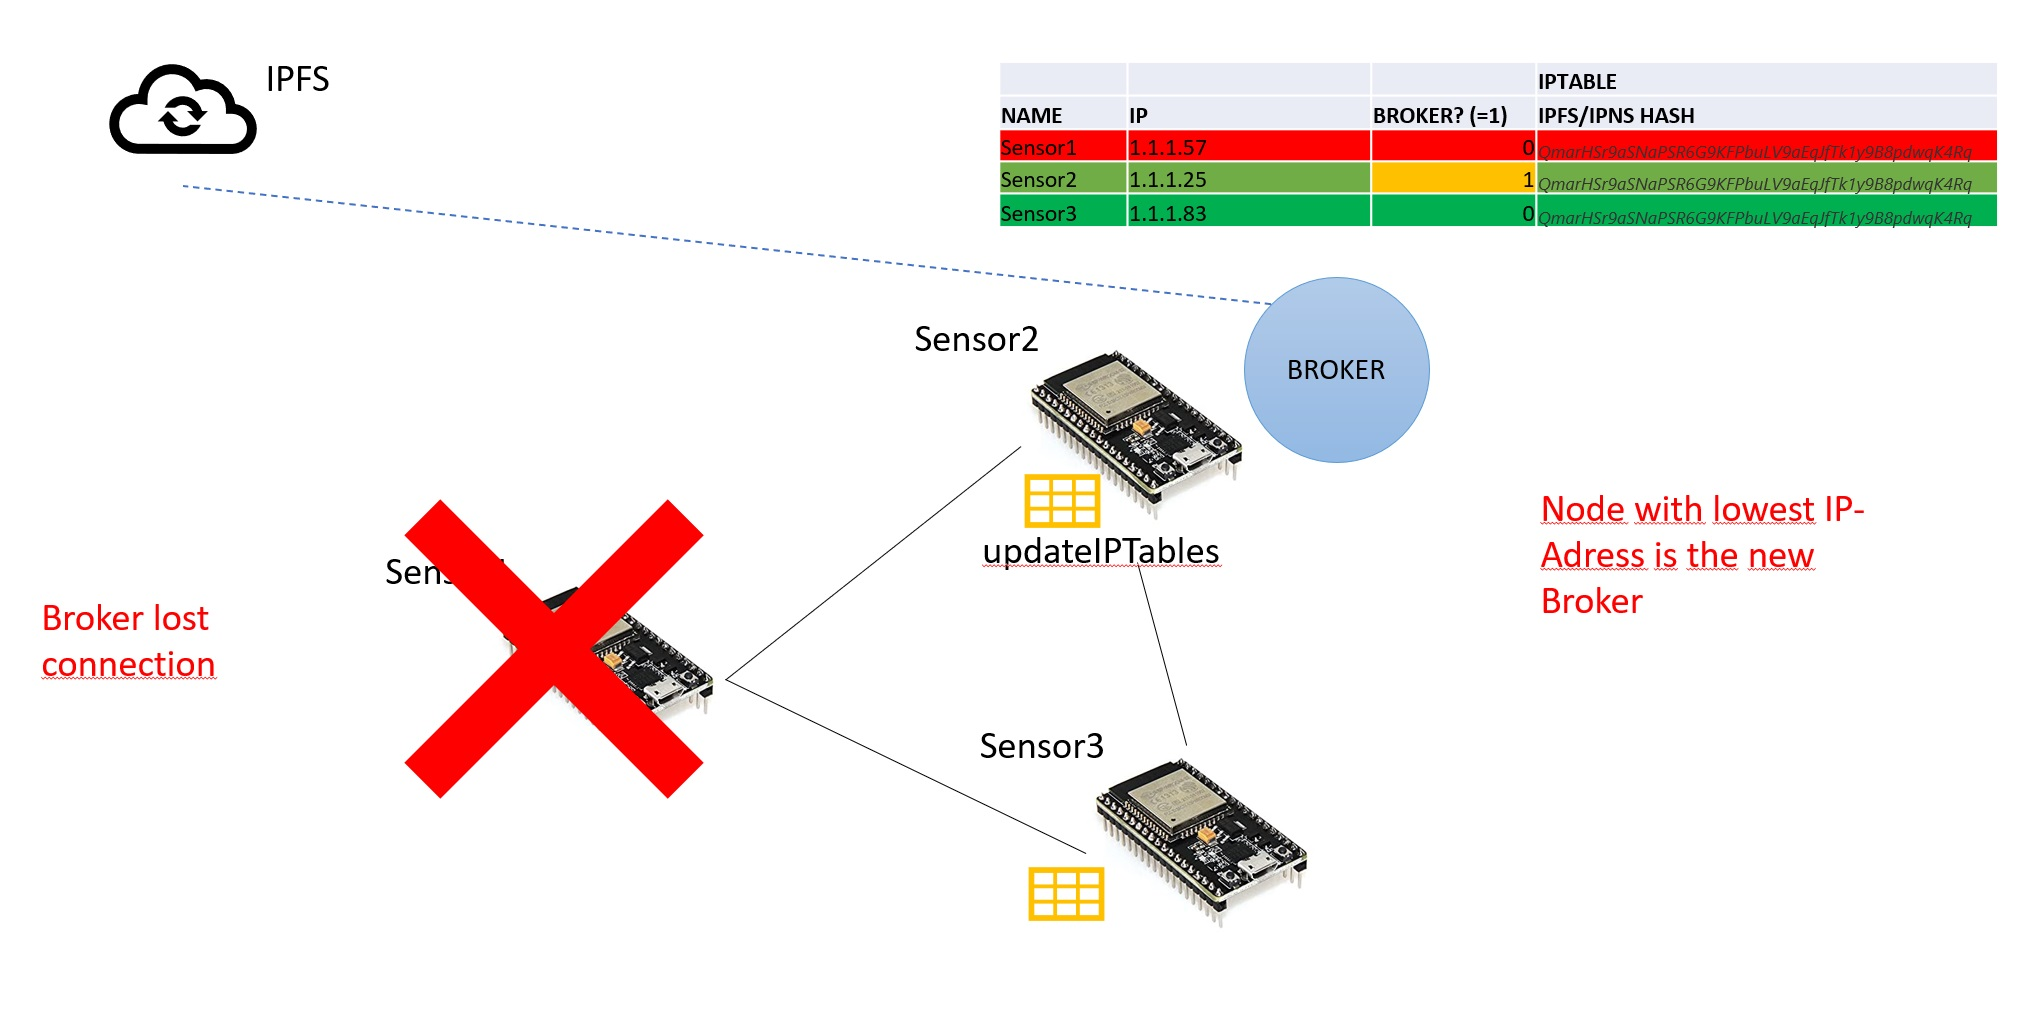
\includegraphics[width=1\linewidth]{Porposal/Bilder/Bild4.jpg}
    \caption{Der Broker verliert die Verbindung und ein neuer Broker wird bestimmt. }
    \label{fig:statemachine}
\end{figure}

Sobald der abgestürzte Client/Broker die Verbindung wieder aufbauen konnte, erhält er die aktuelle IP-Tabelle aus dem Cloudspeicher und verbindet sich mit dem neuen Broker.

\begin{figure}[h]
    \centering
    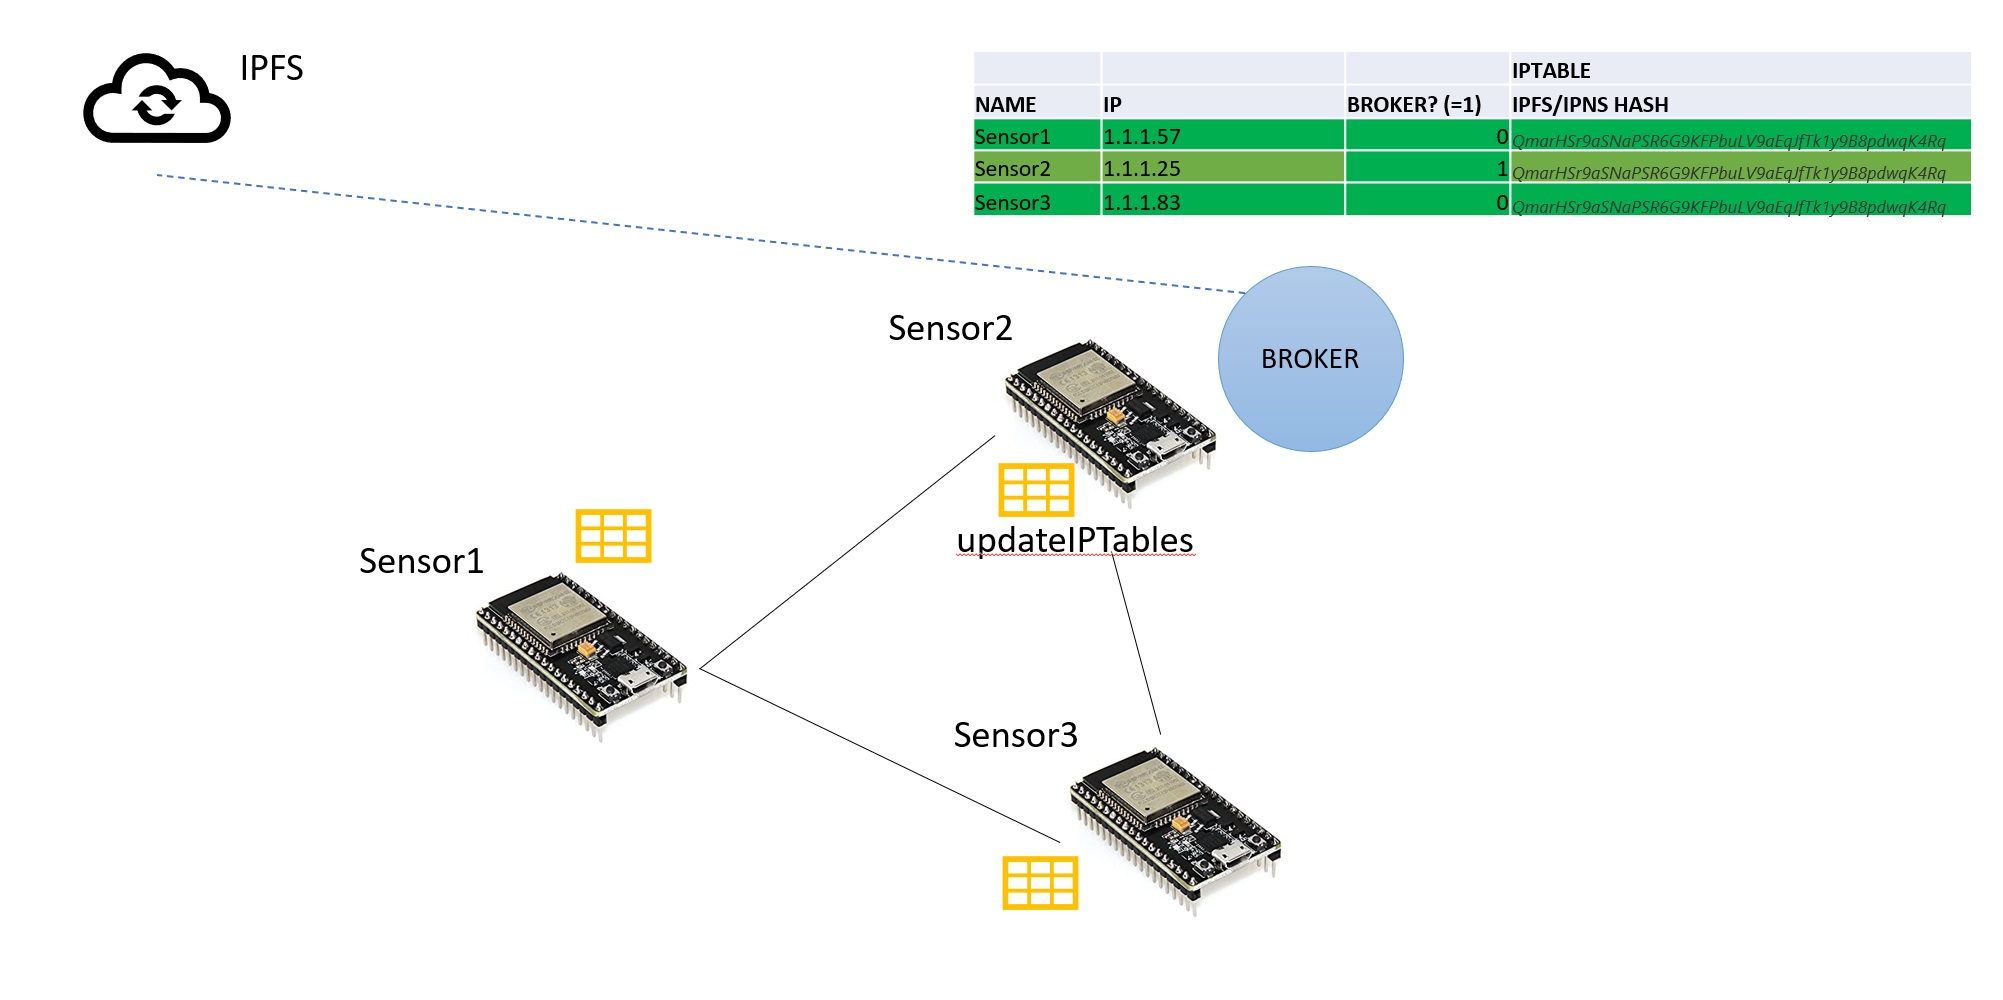
\includegraphics[width=1\linewidth]{Porposal/Bilder/Bild5.jpg}
    \caption{Der ehemalige Broker ist jetzt Client}
    \label{fig:statemachine}
\end{figure}

\section{Stand der Technik / Related Work}
\end{document}

